% Native editable composition from verified, unchanged IDE images.
\par
\begin{figure}[htbp]
  \centering
  \sbox0{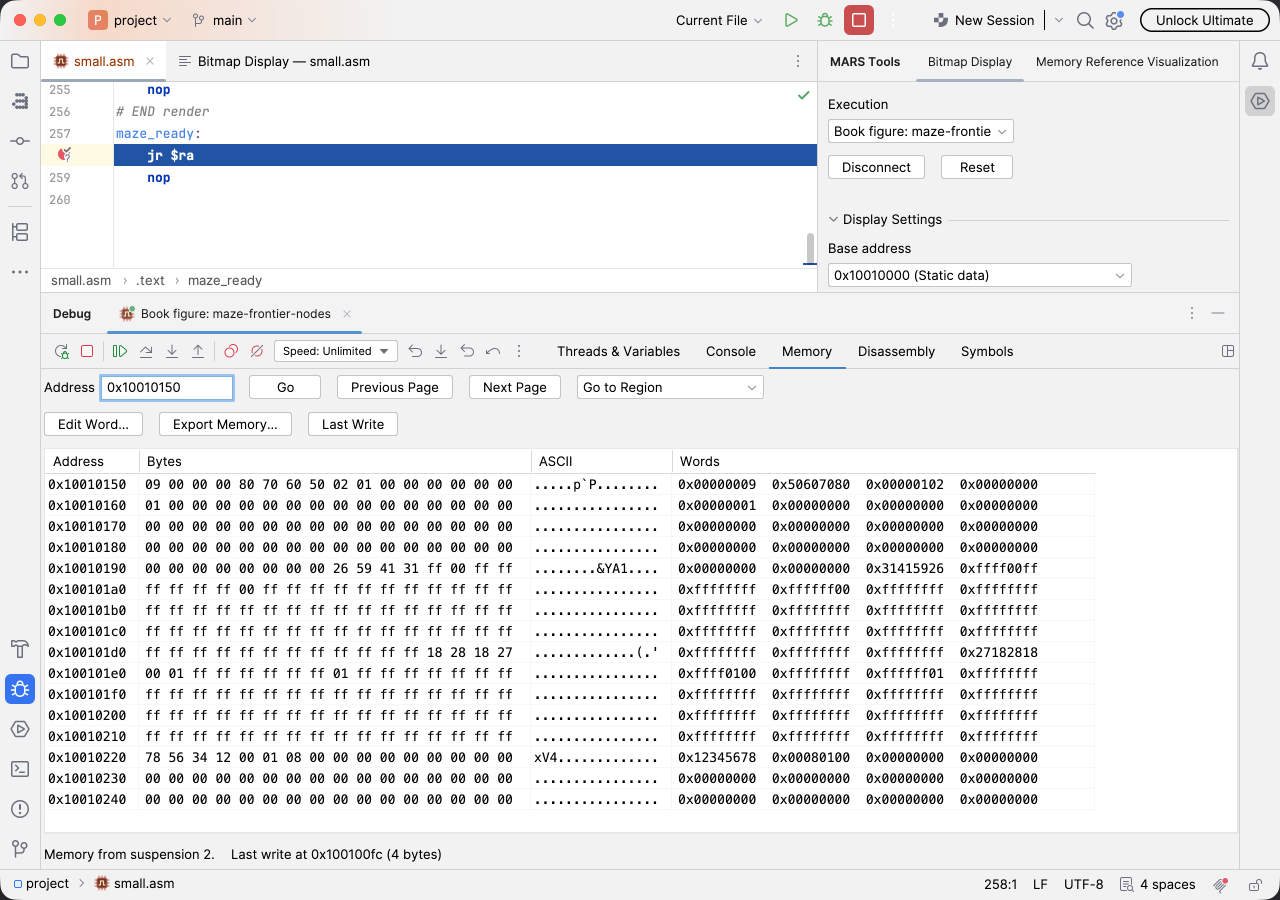
\includegraphics[artifact]{packages/010-maze-explorer/captures/f02-frontier/nodes.png}}
  \sbox2{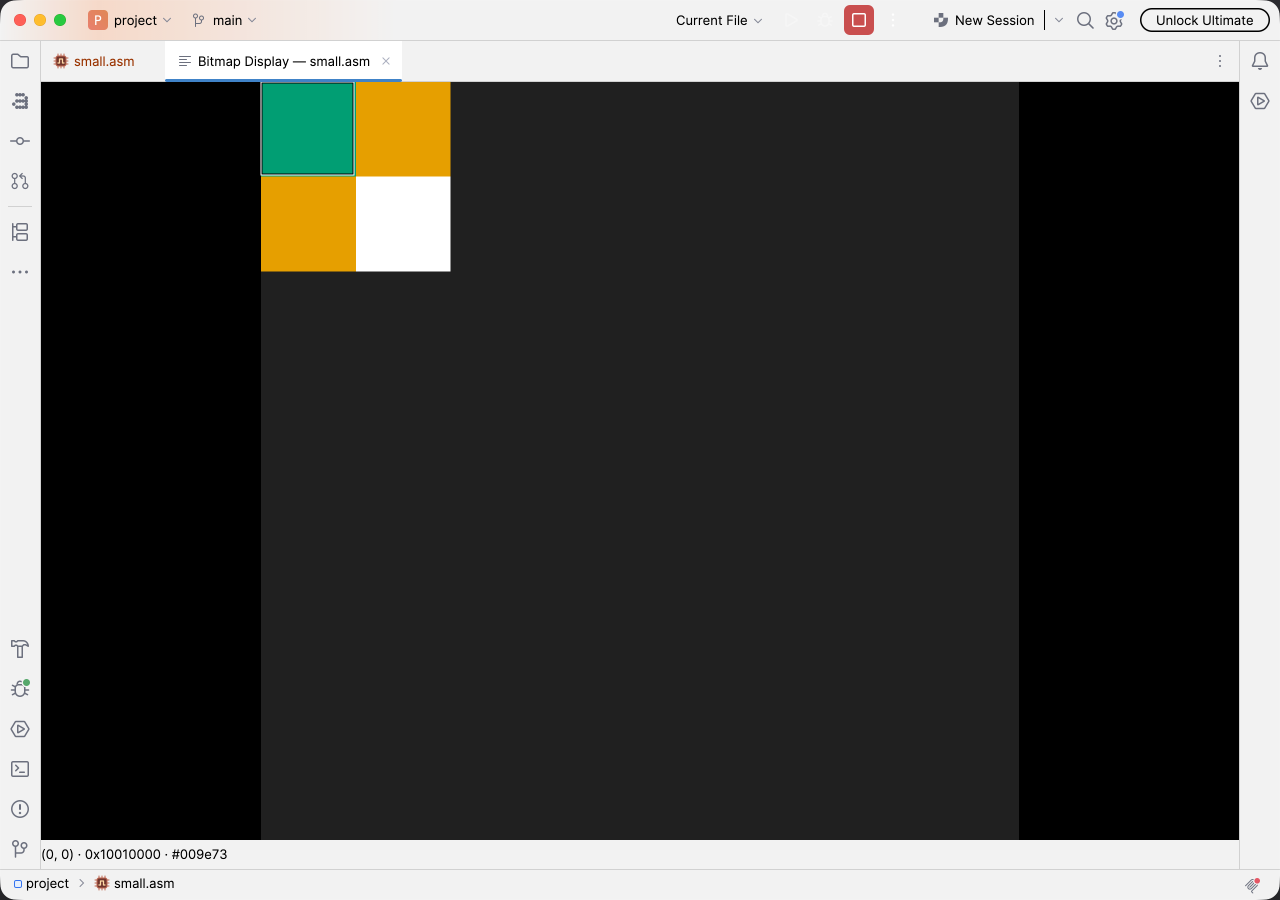
\includegraphics[artifact]{packages/010-maze-explorer/captures/f02-frontier/bitmap.png}}
  \sbox4{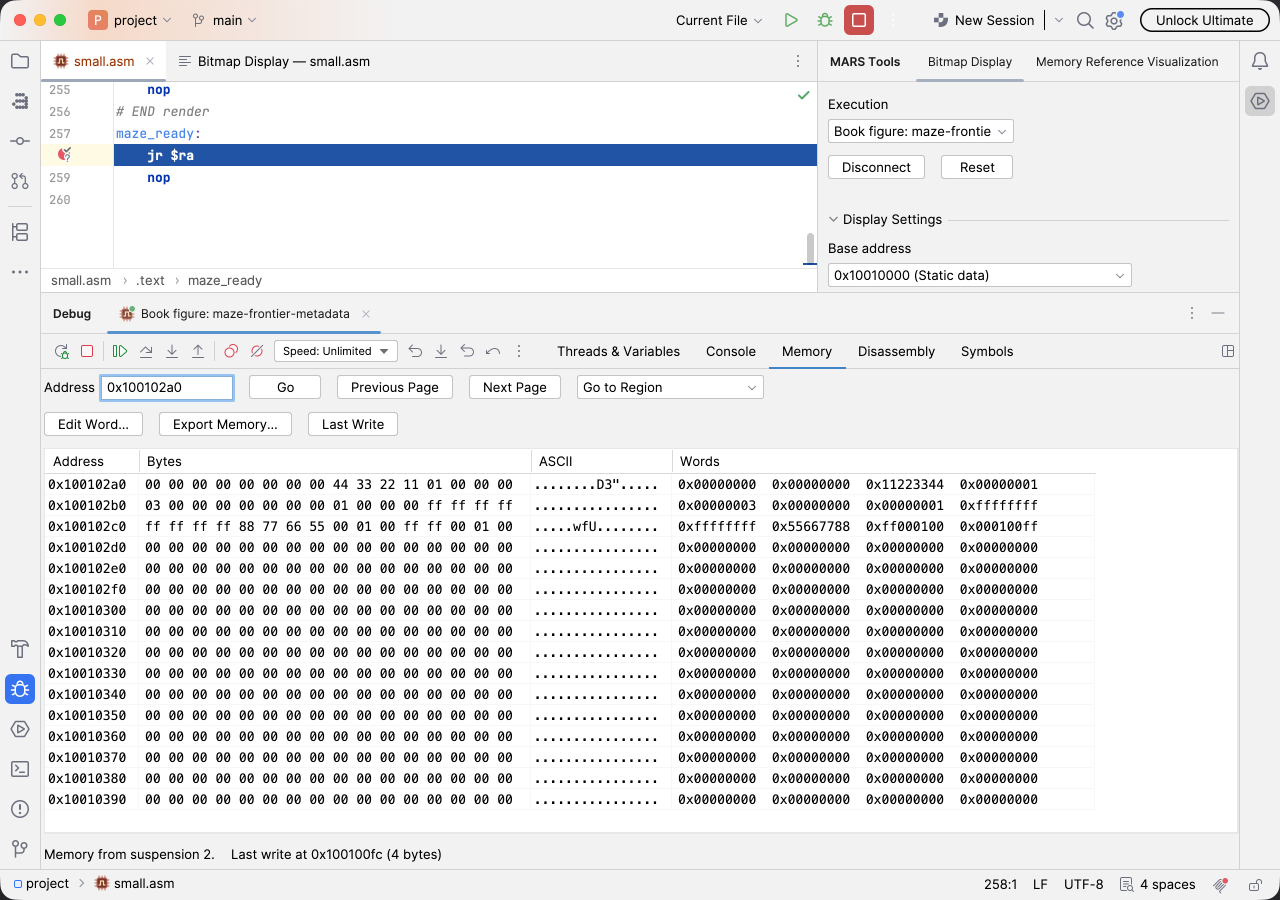
\includegraphics[artifact]{packages/010-maze-explorer/captures/f02-frontier/metadata.png}}
  \edef\MARSfrontiersourceLeft{\the\dimexpr0.036718750\wd0\relax}
  \edef\MARSfrontiersourceBottom{\the\dimexpr0.811111111\ht0\relax}
  \edef\MARSfrontiersourceRight{\the\dimexpr0.611718750\wd0\relax}
  \edef\MARSfrontiersourceTop{\the\dimexpr0.111111111\ht0\relax}
  \edef\MARSfrontierstateLeft{\the\dimexpr0.034375000\wd0\relax}
  \edef\MARSfrontierstateBottom{\the\dimexpr0.422222222\ht0\relax}
  \edef\MARSfrontierstateRight{\the\dimexpr0.584375000\wd0\relax}
  \edef\MARSfrontierstateTop{\the\dimexpr0.497777778\ht0\relax}
  \edef\MARSfrontierlinksLeft{\the\dimexpr0.034375000\wd0\relax}
  \edef\MARSfrontierlinksBottom{\the\dimexpr0.236666667\ht0\relax}
  \edef\MARSfrontierlinksRight{\the\dimexpr0.584375000\wd0\relax}
  \edef\MARSfrontierlinksTop{\the\dimexpr0.616666667\ht0\relax}
  \edef\MARSfrontierplotLeft{\the\dimexpr0.203906250\wd2\relax}
  \edef\MARSfrontierplotBottom{\the\dimexpr0.066666667\ht2\relax}
  \edef\MARSfrontierplotRight{\the\dimexpr0.203906250\wd2\relax}
  \edef\MARSfrontierplotTop{\the\dimexpr0.091111111\ht2\relax}
  \edef\MARSfrontiermemoryLeft{\the\dimexpr0.034375000\wd4\relax}
  \edef\MARSfrontiermemoryBottom{\the\dimexpr0.398888889\ht4\relax}
  \edef\MARSfrontiermemoryRight{\the\dimexpr0.584375000\wd4\relax}
  \edef\MARSfrontiermemoryTop{\the\dimexpr0.497777778\ht4\relax}
  \begin{tikzpicture}[alt={Five annotated details after processing start cell zero. Its state is two, meaning processed. Cells one and eight are frontier with state one; cell nine is unseen. Both newly discovered parents are zero and both distances are one. Head is one, tail three, current zero, phase one. Result and route length remain minus one.}]
    \node[anchor=north west,inner sep=0,font=\small\bfseries] (source-title) at (6mm,0) {Next instruction: return from the renderer};
    \node[anchor=north west,inner sep=0] (source) at ([yshift=-1mm]source-title.south west) {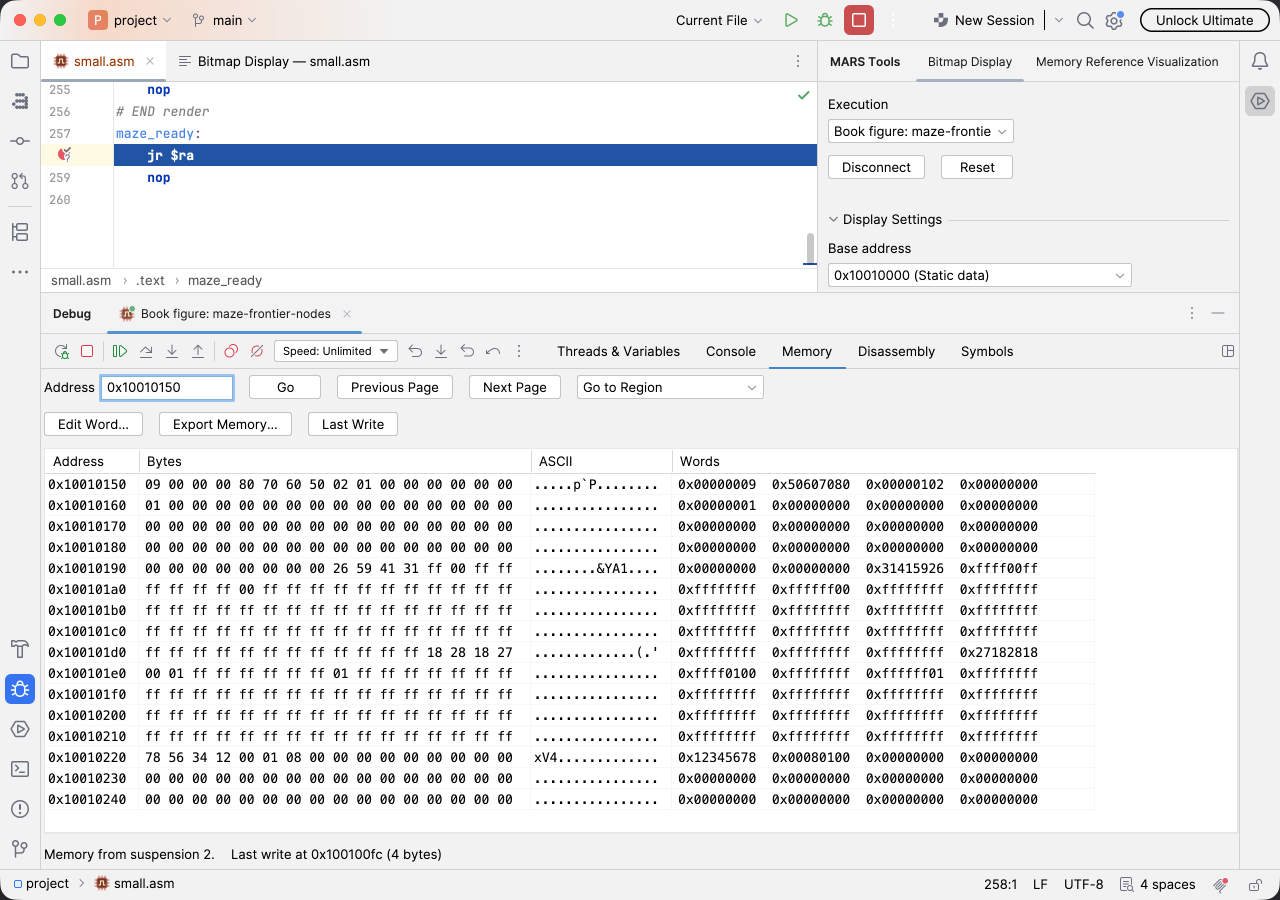
\includegraphics[width=0.7\linewidth,artifact,trim={\MARSfrontiersourceLeft{} \MARSfrontiersourceBottom{} \MARSfrontiersourceRight{} \MARSfrontiersourceTop{}},clip]{packages/010-maze-explorer/captures/f02-frontier/nodes.png}};
    \begin{scope}[shift={(source.south west)},x={($(source.south east)-(source.south west)$)},y={($(source.north west)-(source.south west)$)}]
      \draw[black,line width=0.7pt] (0.153333333,0.057142857) rectangle (0.326666667,0.371428571);
      \node[draw=black,fill=white,circle,inner sep=1.5pt,font=\footnotesize] at ($(0.153333333,0.371428571)+(-3mm,0)$) {1};
    \end{scope}
    \node[anchor=north west,inner sep=0,font=\small\bfseries] (state-title) at ([yshift=-1mm]source.south west) {State bytes for the first two rows};
    \node[anchor=north west,inner sep=0] (state) at ([yshift=-1mm]state-title.south west) {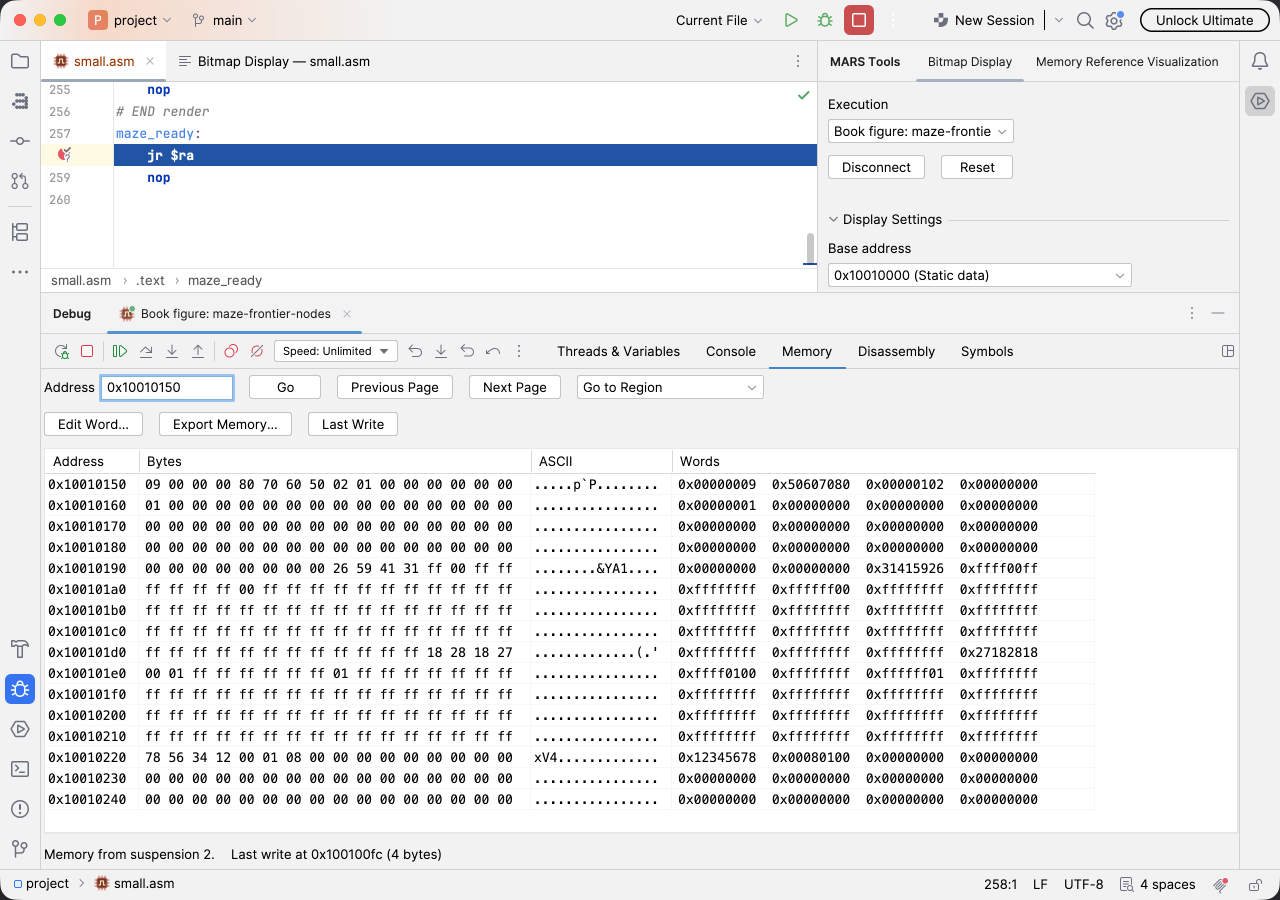
\includegraphics[width=0.78\linewidth,artifact,trim={\MARSfrontierstateLeft{} \MARSfrontierstateBottom{} \MARSfrontierstateRight{} \MARSfrontierstateTop{}},clip]{packages/010-maze-explorer/captures/f02-frontier/nodes.png}};
    \begin{scope}[shift={(state.south west)},x={($(state.south east)-(state.south west)$)},y={($(state.north west)-(state.south west)$)}]
      \draw[black,line width=0.7pt] (0.194672131,0.055555556) rectangle (0.997950820,0.638888889);
      \node[draw=black,fill=white,circle,inner sep=1.5pt,font=\footnotesize] at ($(0.000000000,0.638888889)+(-3mm,0)$) {2};
    \end{scope}
    \node[anchor=north west,inner sep=0,font=\small\bfseries] (links-title) at ([yshift=-1mm]state.south west) {Parents and distances};
    \node[anchor=north west,inner sep=0] (links) at ([yshift=-1mm]links-title.south west) {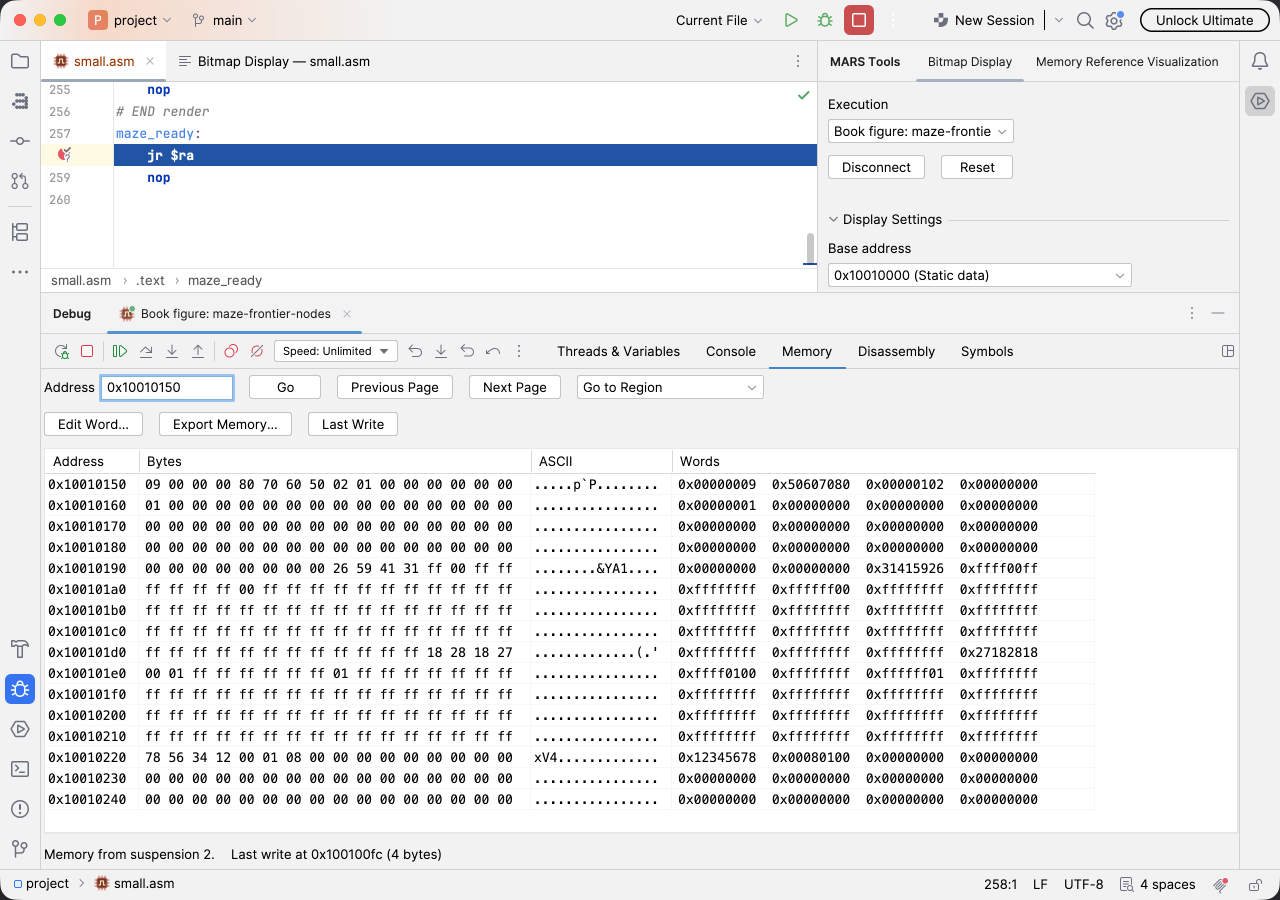
\includegraphics[width=0.6\linewidth,artifact,trim={\MARSfrontierlinksLeft{} \MARSfrontierlinksBottom{} \MARSfrontierlinksRight{} \MARSfrontierlinksTop{}},clip]{packages/010-maze-explorer/captures/f02-frontier/nodes.png}};
    \begin{scope}[shift={(links.south west)},x={($(links.south east)-(links.south west)$)},y={($(links.north west)-(links.south west)$)}]
      \draw[black,line width=0.7pt] (0.194672131,0.022727273) rectangle (0.997950820,0.977272727);
      \node[draw=black,fill=white,circle,inner sep=1.5pt,font=\footnotesize] at ($(0.000000000,0.977272727)+(-3mm,0)$) {3};
    \end{scope}
    \node[anchor=north west,inner sep=0,font=\small\bfseries] (plot-title) at ([xshift=0.67\linewidth]links-title.north west) {Published maze cells};
    \node[anchor=north west,inner sep=0] (plot) at ([yshift=-1mm]plot-title.south west) {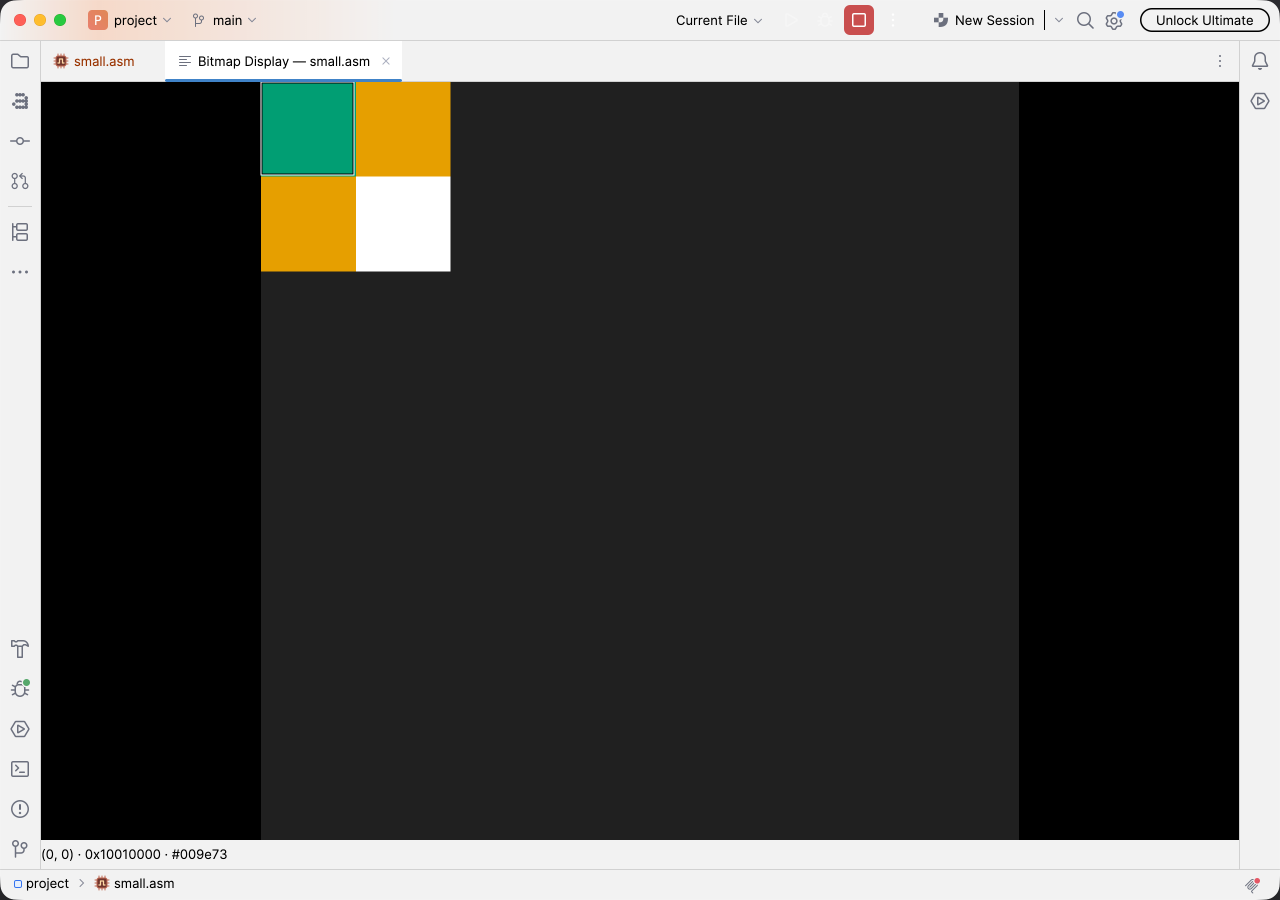
\includegraphics[width=0.27\linewidth,artifact,trim={\MARSfrontierplotLeft{} \MARSfrontierplotBottom{} \MARSfrontierplotRight{} \MARSfrontierplotTop{}},clip]{packages/010-maze-explorer/captures/f02-frontier/bitmap.png}};
    \begin{scope}[shift={(plot.south west)},x={($(plot.south east)-(plot.south west)$)},y={($(plot.north west)-(plot.south west)$)}]
      \draw[black,line width=0.7pt] (0.000000000,0.000000000) rectangle (1.000000000,1.000000000);
      \node[draw=black,fill=white,circle,inner sep=1.5pt,font=\footnotesize] at ($(0.000000000,1.000000000)+(-3mm,0)$) {4};
      \foreach \c in {0,...,7} {\node[anchor=north,font=\scriptsize,inner sep=0] at ({(\c+0.5)/8},-0.035) {\c}; \node[anchor=east,font=\scriptsize,inner sep=0] at (-0.025,{1-(\c+0.5)/8}) {\c};}
      \node[anchor=north,font=\scriptsize,inner sep=0] at (0.5,-0.11) {$x$}; \node[anchor=east,font=\scriptsize,inner sep=0] at (-0.10,0.5) {$y$};
    \end{scope}
    \node[anchor=north west,inner sep=0,font=\small\bfseries] (memory-title) at ([yshift=-9mm]links-title.north west |- plot.south west) {Queue counters and published phase};
    \node[anchor=north west,inner sep=0] (memory) at ([yshift=-1mm]memory-title.south west) {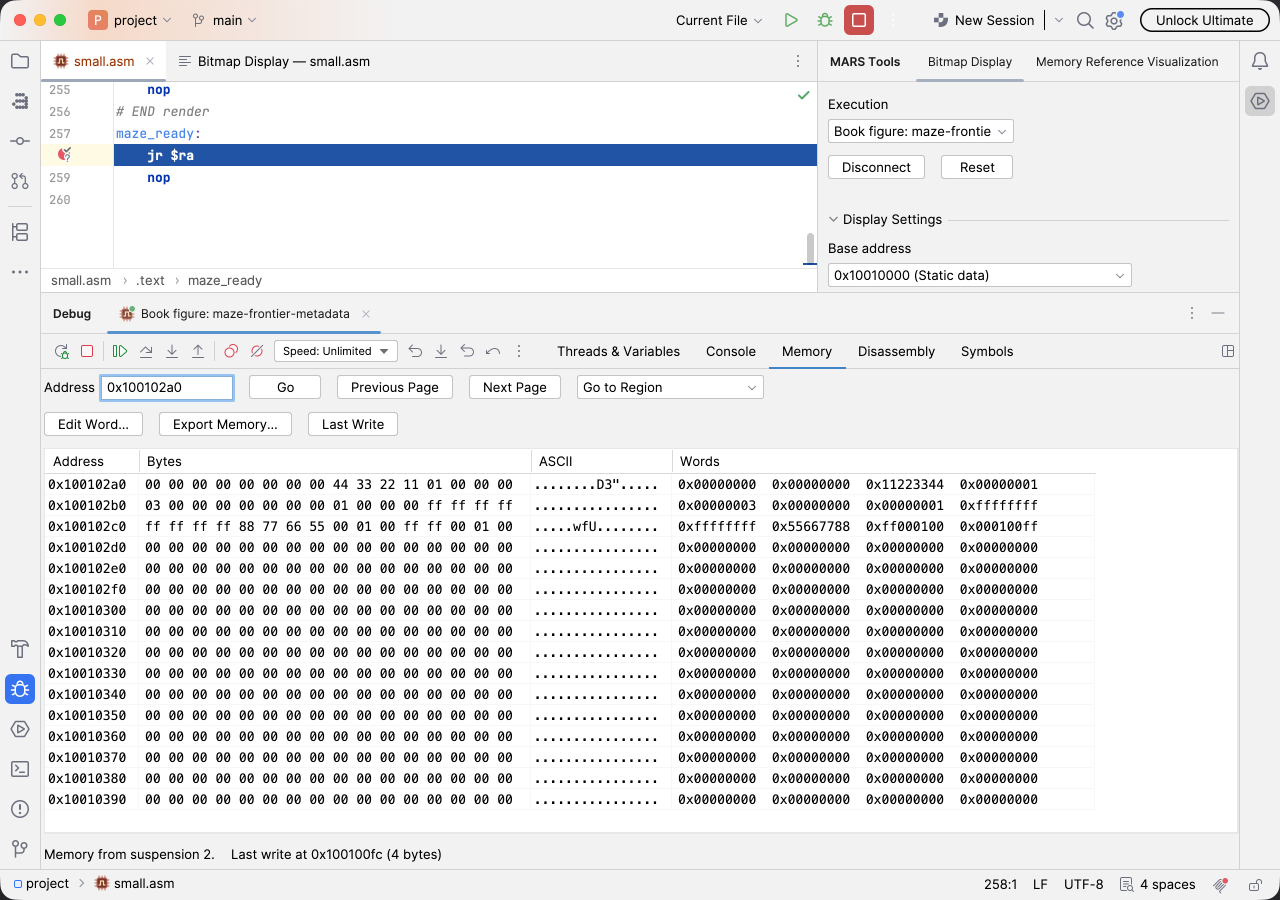
\includegraphics[width=0.78\linewidth,artifact,trim={\MARSfrontiermemoryLeft{} \MARSfrontiermemoryBottom{} \MARSfrontiermemoryRight{} \MARSfrontiermemoryTop{}},clip]{packages/010-maze-explorer/captures/f02-frontier/metadata.png}};
    \begin{scope}[shift={(memory.south west)},x={($(memory.south east)-(memory.south west)$)},y={($(memory.north west)-(memory.south west)$)}]
      \draw[black,line width=0.7pt] (0.194672131,0.043010753) rectangle (0.997950820,0.720430108);
      \node[draw=black,fill=white,circle,inner sep=1.5pt,font=\footnotesize] at ($(0.000000000,0.720430108)+(-3mm,0)$) {5};
    \end{scope}
  \end{tikzpicture}
  \par\smallskip
  \begin{minipage}{\linewidth}
    \small
    \begin{enumerate}
      \item The condition \texttt{\$s5 == 1} selects the first completed expansion at \texttt{maze\_ready}. Neighbor discovery, metadata publication and all 64 pixel stores have finished; the renderer has not returned.
      \item Cell 0 now contains state 2 (processed). Cells 1 and 8 contain state 1 (frontier); cell 9 remains 0. The lower displayed state row starts with cell 8.
      \item Parent bytes for cells 1 and 8 are 0. Their distance bytes are 1. Discovering from start cell 0 establishes these links once; \texttt{ff} still marks cell 9\textquotesingle s unknown parent and distance.
      \item Processed $(0,0)$ is green; frontier cells $(1,0)$ and $(0,1)$ are orange. The remaining open cell $(1,1)$ is white. These classifications also follow from the numeric state bytes, independent of color.
      \item \texttt{head}=1, \texttt{tail}=3 and \texttt{current}=0 publish queue history $[0,1,8]$. The active interval contains cells 1 and 8. Phase is 1; result and length are still $-1$.
    \end{enumerate}
  \end{minipage}
  \caption{Expanding the start discovers two neighbors at distance one.}
  \label{capture:010-maze-explorer-f02-frontier}
  \label{maze-f02-frontier}
\end{figure}
\par
